%% Generate document with:
%% bibtex monad && [xe]latex -src-specials monad
\documentclass{article}

%% Charset & Font:
%\usepackage{ctex}          % CJK
%\usepackage{mathptmx}      % mathptmx font
%\usepackage{tgpagella}     % Palatino, text only
\usepackage{mathpazo}       % Palatino, math & text

\usepackage{amsmath,amsfonts,amssymb,amsbsy}
\usepackage{amsthm}
\usepackage{tikz-cd}

\usepackage[numbers]{natbib}

\input{../../include/usrdef}
\input{../../include/thmenv_e}

%\usetikzlibrary{matrix}
\begin{document}

%\title{\textbf{Norm Minimization of Linear Matrix}}
%\author{
%Rao Fu \\[1em]
%\small{\textit{Center for Systems and Control}} \\
%\small{\textit{Department of Mechanics and Engineering Science}} \\
%\small{\textit{Peking University, Beijing 100871, P.R.China}}
%}

%\title{\Huge{\textbf{LECTURE NOTES}} \\ \Huge{\textbf{ON}} \\ \Huge{\textbf{MATHEMATICS}} \\[1em] {Note on Monad}}

\title{\textbf{Lecture Notes on Mathmatics} \\[1em] What the Hell is Monad ?
{\footnote{\texttt{Document No. 2017-09-22-001}}}
{\footnote{\copyright \texttt{2017 - 2017 by texacker.org. All rights reserved.}}}
}

\author{%
%\textit{texacker.org}
\small{\textit{rao.fu}}\thanks{\texttt{http://www.texacker.org/\~{}furao}} \\ \small{\textit{texacker.org}}
}
\date{\today}

\maketitle

\section{Categories}
\subsection{Categories}
\begin{defn}[{\cite{AS10}}]
%\label{defn:63}
A category consists of the following data:
\begin{itemize}
\item
Objects: $A,B,C,\dotsc$
\item
Arrows: $f,g,h,\dotsc$
\item
For each arrow $f$, there are given objects
\[
dom(f),\quad cod(f)
\]
called the \emph{domain} and \emph{codomain} of $f$. We write
\[
f: A \rightarrow B
\]
to indicate that $A = dom(f)$ and $B = cod(f)$.
\item
Given arrows $f: A \rightarrow B$ and $g: B \rightarrow C$, that is, with
\[
dom(f) = cod(g)
\]
there is given an arrow
\[
g \circ f: A \rightarrow C
\]
called the \emph{composite} of $f$ and $g$.
\item
For each object $A$, there is given an arrow
\[
1_{A}: A \rightarrow A
\]
called the \emph{identity} arrow of $A$.
\end{itemize}
These data are required to satisfy the following laws:
\begin{itemize}
\item
Associativity:
\[
h \circ ( g \circ f ) = ( h \circ g ) \circ f
\]
for all $f : A \rightarrow B$, $g : B \rightarrow C$, $h : C \rightarrow D$.
\item
Unit:
\[
f \circ 1_{A} = f = 1_{B} \circ f
\]
for all $f : A \rightarrow B$.
\end{itemize}
\end{defn}

%\begin{gather}
%%\label{equ:SDP.primal}
%\min \gamma \\
%s.t.\,\,
%\begin{bmatrix}
%\gamma I & A \\
%A^T      & \gamma I
%\end{bmatrix}
%\ge 0 \notag
%\end{gather}
%therefore the minimization of $\norm{P - P_0}$ with given $P_0$
%has the form:
%\begin{gather}
%%\label{equ:SDP.primal}
%\min \gamma \\
%s.t.\,\,
%\begin{bmatrix}
%\gamma I    & P - P_0 \\
%P^T - P_0^T & \gamma I
%\end{bmatrix}
%\ge 0 \notag
%\end{gather}

\subsection{Functors}
\begin{defn}[{\cite{AS10}}]
A functor
\[
F: \mathbf{C} \rightarrow \mathbf{D}
\]
between categories $\mathbf{C}$ and $\mathbf{D}$ is a mapping of objects to objects and arrows to arrows,
in such a way that
\begin{enumerate}
\item
\[
F(f:A \rightarrow B) = F(f):F(A) \rightarrow F(B)
\]
\item
\[
F(1_{A}) = 1_{F(A)}
\]
\item
\[
F(f \circ g) = F(f) \circ F(g)
\]
\end{enumerate}
That is, $F$ preserves \emph{domain}s and \emph{codomain}s, \emph{identity} arrows, and \emph{compostion}.
\end{defn}

\section{Naturality}
\subsection{Natural Transformations}
\begin{defn}[{\cite{AS10}}]
For categories $\mathbf{C}$, $\mathbf{D}$ and functors
\[
F,G: \mathbf{C} \rightarrow \mathbf{D}
\]
a \emph{natural transformation} $\vartheta: F \rightarrow G$ is a family of arrows in $\mathbf{D}$
\[
(\vartheta_{A}: FA \rightarrow GA)_{A \in \mathbf{C_0}}
\]
such that, for any $f: A \rightarrow A'$ in $\mathbf{C}$, one has
\[
\vartheta_{A'} \circ F(f) = G(f) \circ \vartheta_{A}
\]
that is, the following commutes:
%\[
%\begin{tikzcd}
%A\arrow[bend left]{r}\arrow[bend right]{r}&B
%\end{tikzcd}
%\]
\[
\begin{tikzcd}[row sep=huge, column sep=huge]
FA \arrow[r, "\vartheta_{A}"] \arrow[d, "Ff"'] & GA \arrow[d, "Gf"] \\
FA' \arrow[r, "\vartheta_{A'}"]                & GA'
\end{tikzcd}
\]
\end{defn}

\section{Adjoints}

\subsection{Freeness}
\begin{exam}[{\cite{AM75}}]
The monoid $A=(X^{*}, conc, \Lambda)$
\end{exam}

\begin{lem}[{\cite{AM75}}]
A monoid $A$
\end{lem}

\begin{defn}[\cite{AM75}, Definition~7.2.4]
Let $G: \mathbf{A} \rightarrow \mathbf{B}$ be any functors, and $B$ an object of $\mathbf{B}$.
We say the pair $(A, \eta)$, where $A$ is an object of $\mathbf{A}$ and $\eta: B \rightarrow GA$ is a morphism of $B$,
is \emph{free over $B$ with respect to $G$} just in case $\eta: B \rightarrow GA$ has the couniversal property that
given any morphism $f: B \rightarrow GA'$ with $A'$ any object of $A$,
there exists a unique $\mathbf{A}$-morphism $\psi: A \rightarrow A'$ such that
\[
\begin{tikzcd}[row sep=huge, column sep=huge]
B \arrow[r, "\eta"] \arrow[rd, "f"'] & GA \arrow[d, dashrightarrow, "G\psi"] \\
                                     & GA'
\end{tikzcd}
\qquad
\begin{tikzcd}[row sep=huge, column sep=huge]
A \arrow[d, dashrightarrow, "\psi"] \\
A'
\end{tikzcd}
\]
\end{defn}

\subsection{Adjoints}

\subsection{Adjunctions}

\section{Monads}

\subsection{Monads}

%\subsubsection{F-Algebras}

\subsection{Eilenberg-Moore Category}
%\begin{tikzpicture}
%  \matrix (m) [matrix of math nodes,row sep=3em,column sep=4em,minimum width=2em]
%  {
%     F_t(x) & F(x) \\
%     A_t & A \\};
%  \path[-stealth]
%    (m-1-1) edge node [left] {$\mathcal{B}_X$} (m-2-1)
%            edge [double] node [below] {$\mathcal{B}_t$} (m-1-2)
%    (m-2-1.east|-m-2-2) edge node [below] {$\mathcal{B}_T$}
%            node [above] {$\exists$} (m-2-2)
%    (m-1-2) edge node [right] {$\mathcal{B}_T$} (m-2-2)
%            edge [dashed,-] (m-2-1);
%\end{tikzpicture}

\[
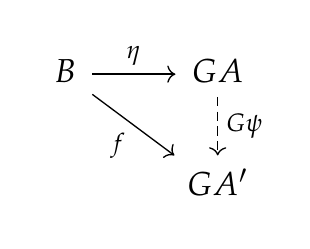
\begin{tikzpicture}[baseline= (a).base]
\node[scale=1.2] (a) at (0,0){
\begin{tikzcd}
B \arrow[r, "\eta"] \arrow[rd, "f"'] & GA \arrow[d, dashrightarrow, "G\psi"] \\
                                     & GA'
\end{tikzcd}
};
\end{tikzpicture}
\qquad
\begin{tikzpicture}[baseline= (a).base]
\node[scale=1.2] (a) at (0,0){
\begin{tikzcd}
A \arrow[d, dashrightarrow, "\psi"] \\
A'
\end{tikzcd}
};
\end{tikzpicture}
\]

\subsection{Kleisli Category}

%\appendix
\section{Algebraic Theories}
%\subsection{Free Algebra}

\section{Monad in Haskell}
\subsection{Kleisli Triples}

It's well known that the structured singular value (SSV) method,
which was introduced by {\citet{PBC91}} and {\citet{AS10}},
is one of most effective approach to deal with robustness analysis and controller synthesis for systems
subject to mixed un-modelled dynamic uncertainty and parametric uncertainty.
However, except for some special cases, most of the currently available approaches for SSV analysis and synthesis require
frequency sweeping which is computational costly and prone to erroneous answers
when the SSV curve is discontinuous.
Besides, the curve-fitting step involved in the synthesis procedure makes these methods computationally intractable.
To overcome these drawbacks, some newly improved approaches were presented recently by using convex optimization approaches,
such as {\citep{BirddeMoor96:Algebra}} and {\citep{AV12}}.
Comparing with the conventional frequency domain method,
the convex optimization approaches are generally of a better numerical property
by virtue of the interior-point polynomial time algorithms{\citep{AM75}} and require no frequency sweep.
But unfortunately, none of these approaches is capable of solving large-scale SSV test
since they are all exponentially complex.
%the readily available convex optimization methods in literature,
%such as that proposed by Chen and Sugie in 1998, are exponentially complex and therefore
%unable to solve large-scale SSV analysis and synthesis problem.
Moreover, most of the widely used numerical algorithms,
such as the Projective Algorithm presented by {\citet{MLS98}},
are also incapable to handle large-scale convex optimization problems.

Over the past few years, I have made several contributions in solving large-scale SSV analysis and synthesis
using convex optimization method.
By using S-procedure techniques, I have presented a new convex optimization-based
approach for the large-scale mixed SSV analysis and synthesis problem.
Based on the analysis of currently available methods when dealing with large-scale SSV analysis and synthesis problem,
I derived a sufficient condition of the feasibility of robust LMI (Linear Matrix Inequality)
by using S-procedure, and consequently, a less computational expensive SSV upper bound for
a large-scale dynamic system was presented.
The proposed approach {\citep{BGM15}} which is polynomial complex bases on state-space and requires no frequency sweeping{\citep{MEG76}}.
Based on this result, I also gave an LMI criterion for the existence of a full-state feedback SSV controller{\citep{RDE85}}.

%  Revision Log:
%
%  如果有一个 Monad (T, \mu, \eta),则可得到
%  1. 一个 \emph{$T$-Algebra Category} $C^{T}$ (其每个 objects 是 $T$-Algebra)
%  2. 一对 Adjoints(即存在 unit, counit)

%2017-12-06
%  说一个 functor T 是一个 monad,意味着这个 functor T 可以任意类型(表达式)A 为基
%  构造出一个新类型(表达式)TA,并且:

%  1. 这个新类型(表达式)TA 与原来类型(表达式)A 保持某种结构相似性(\eta),
%  2. 同时这个新类型(表达式)TA 上还具有某种“代数”运算(\mu)

%  同时 \mu, \eta 还是相容的。

%2017-12-07
%  free algebra 无求值函数,定义求值函数的为 varieties。

%  Monad means an algebraic theory ?

%2017-12-09
%  \mu, \eta 的形式是成为一个 algebra 的充要条件,
%  而 \mu, \eta 的具体定义则决定了是一个什么样的 algebra:
%  1. \eta : it's free, and there is an unambiguous way of inclusion of generators
%  2. \mu  : an unambiguous way of evaluation

\bibliographystyle{unsrtnat}
\bibliography{../../bib/bib_art,../../bib/bib_book,../../bib/bib_cnf,../../bib/bib_man,../../bib/bib_tech,../../bib/bib_proc}

\end{document}
